\documentclass[notitlepage]{revtex4-1}

\usepackage{graphicx}
\usepackage[margin=5pt]{subfig}
\usepackage[usenames]{color}
% \usepackage{xspace}
\definecolor{darkgreen}{rgb}{0.00,0.50,0.25}
\definecolor{darkblue}{rgb}{0.00,0.00,0.67}
\newcommand{\figref}[1]{Fig.~\ref{#1}}
\usepackage[breaklinks,pdftitle={ZeroDB whitepaper}, pdfauthor={Michael Egorov},colorlinks,urlcolor=blue,citecolor=darkgreen,linkcolor=darkblue]{hyperref}
\usepackage[usenames]{color}
\graphicspath{{pdf/}}

\begin{document}

\title{ZeroDB whitepaper}

\author{M. Egorov}
\email{michael@zerodb.io}
\author{M. Wilkison}
\email{maclane@zerodb.io}

\begin{abstract}
ZeroDB is an end-to-end encrypted database that enables clients to operate on (search, sort, query, and share) encrypted data without exposing encryption keys or cleartext data to the database server.
The familiar client-server architecture remains, but query logic and encryption keys are pushed client-side.
Since the server has no insight into the nature of the data, the risk of a server-side data breach is eliminated.
Even if adversaries successfully infiltrate the server, they will not have access to the cleartext data.

ZeroDB provides end-to-end encryption while maintaining much of the functionality expected of a modern database, such as full-text search, sort, and range queries.
Additionally, ZeroDB uses proxy re-encryption and/or delta key technology to enable secure, granular sharing of encrypted data without exposing keys to the server and without a risk of sharing the same encryption key between all users of the database.
\end{abstract}

\date{\today}
\maketitle

\section{Introduction}

Review of existing systems needed:~\cite{cipherbase}~\cite{cryptdb}~\cite{gentry}

\section{Query protocol}

Basis of the end-to-end encrypted query protocol is following.
The client interacts with the server during the execution of a query over a series of multiple round trips.
An encrypted index is stored on the server as a B-Tree, and the client traverses this index remotely to retrieve the necessary encrypted records.
Buckets which the index consists of are encrypted before being uploaded to the server and decrypted only on the side of the client.

\subsection{Keyword search}
\begin{figure}
	\begin{center}
        \subfloat{\label{fig:tree-traversal}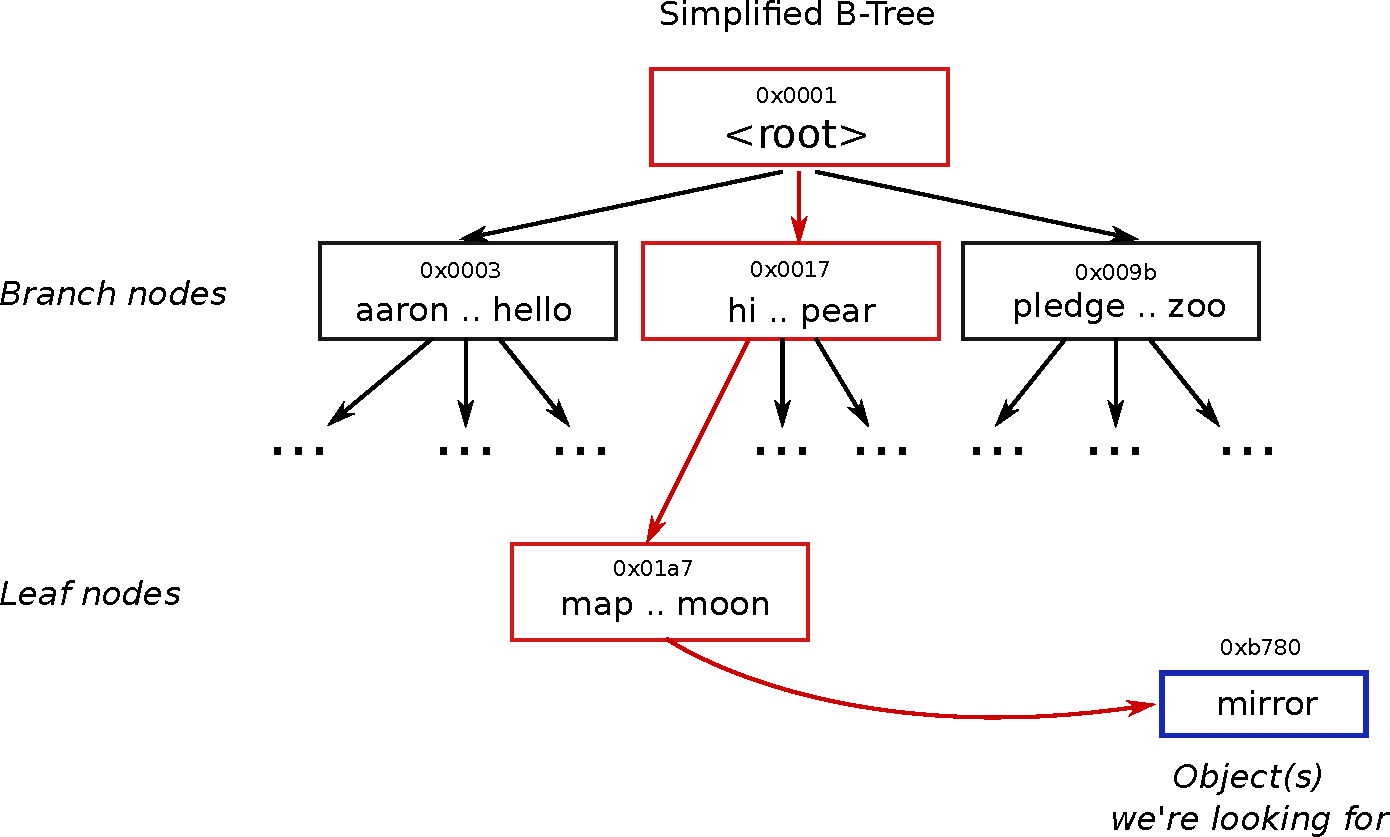
\includegraphics[width=0.47\columnwidth]{btree-traverse.pdf}}
        \qquad
		\subfloat{\label{fig:communication}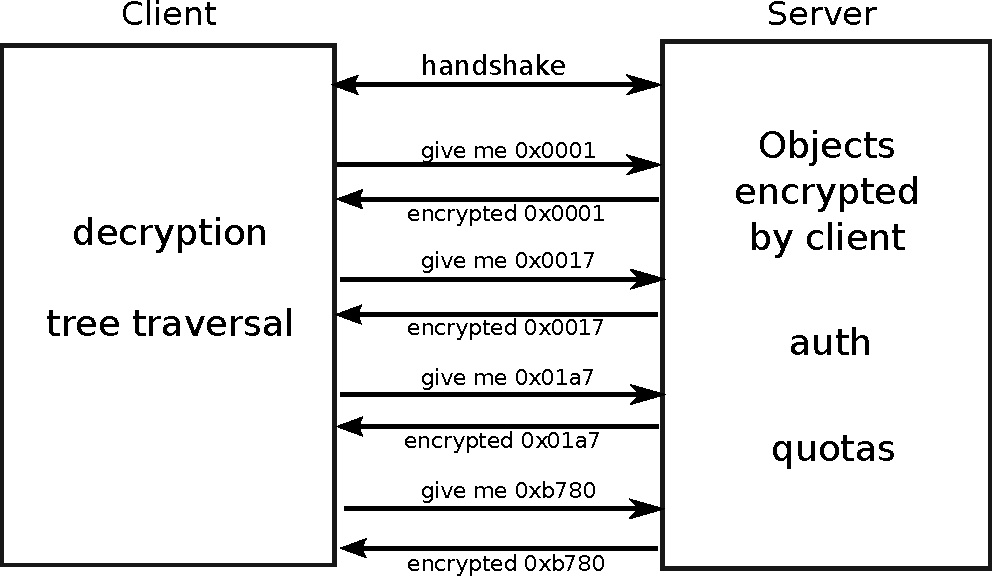
\includegraphics[width=0.47\columnwidth]{protocol.pdf}}
	\end{center}
    \caption[Search protocol using an example of keyword search]{
        \subref{fig:tree-traversal} Encrypted index traversal example (simple keyword search).
		\subref{fig:communication} Sequence of client requests for traversal of the example index.
	}
	\label{fig:btree-protocol}
\end{figure}

In ZeroDB, indexes are structured as B-Trees~\figref{fig:tree-traversal}.
A B-Tree consists of buckets, each of which can be either a root, branch, or leaf node.
The leaf nodes of a tree point to the actual objects being stored.
Thus, searching the database is a simple tree traversal.

In order to make the database end-to-end encrypted yet still capable of performing queries, the client encrypts the buckets (at the time of creation or modification).
The server, which stores the buckets, never knows the encryption key used.
The objects referenced by the leaf nodes of the B-Tree indexes are also encrypted client-side.
As a result, the server does not know how individual objects are organized within the B-Tree or whether they even belong to an index at all.
Since ZeroDB is encryption agnostic, probabilistic encryption can be used so that the server cannot compare objects, not even for equality.

When a client performs a query, it asks the server to return buckets of the tree as it traverses the index remotely~\figref{fig:communication}.
Buckets can be cached client-side so that subsequent queries do not make unnecessary network calls.

The server cares about data replication, multi-version concurrency, object locking, user authentication, quotas etc.
The client performs encryption/decryption and query logic.

\subsection{Range queries}

\begin{figure}
	\begin{center}
        \subfloat{\label{fig:range-query-iter}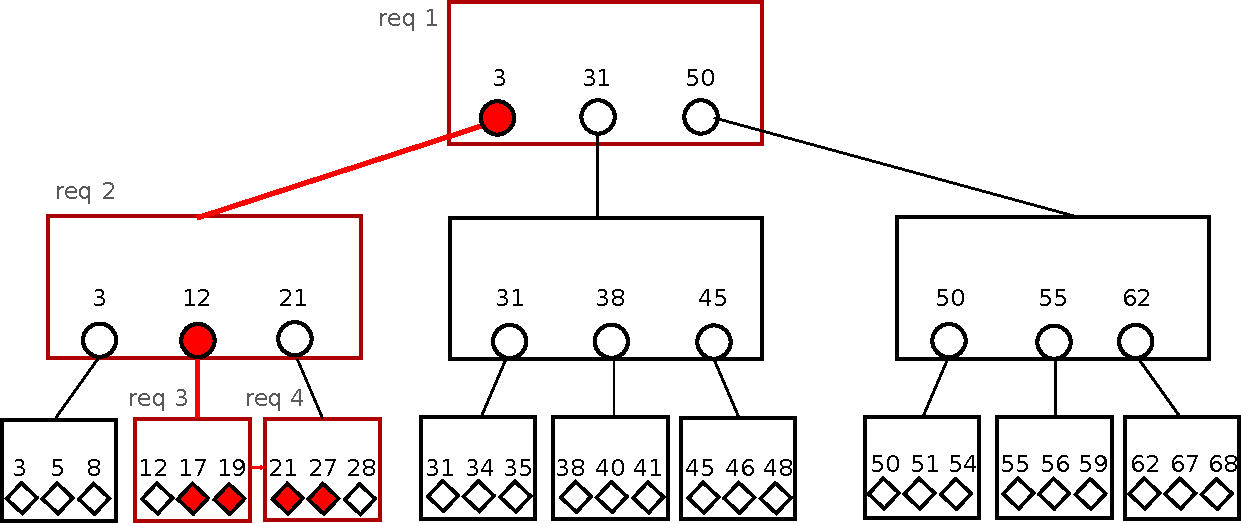
\includegraphics[width=0.47\columnwidth]{range-query-iter.pdf}}
        \qquad
        \subfloat{\label{fig:range-query-star}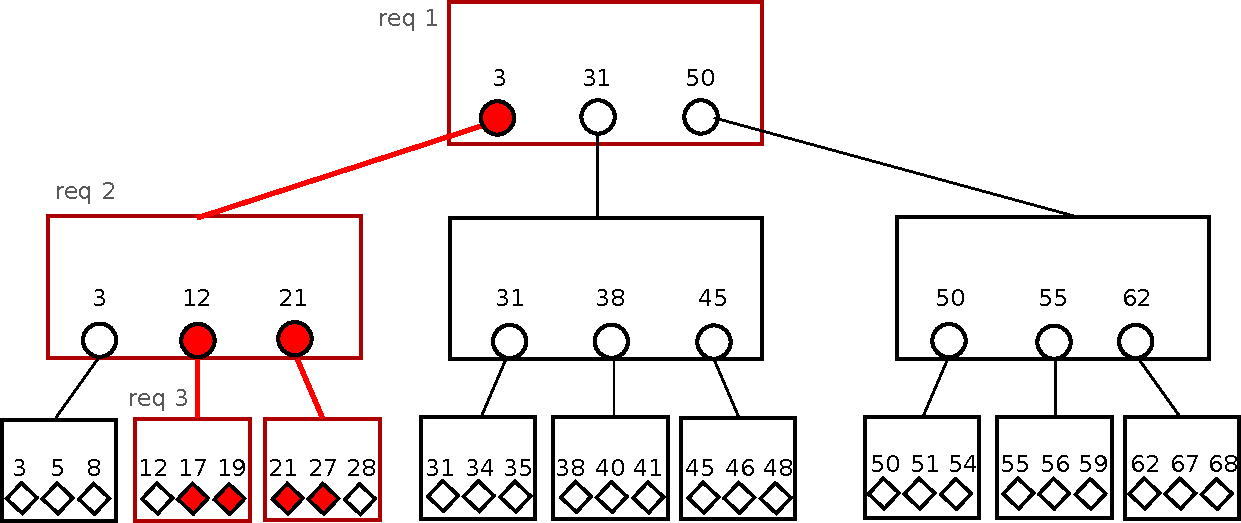
\includegraphics[width=0.47\columnwidth]{range-query-star.pdf}}
	\end{center}
	\caption[Range queries]{
        \subref{fig:range-query-iter} Range query searching for objects with a property $16 \le weight$, $limit=4$ (takes 4 requests w/o cache).
        \subref{fig:range-query-star} Range query which fetches \emph{all} objects  with $16 \le weight \le 27$ (takes 3 requests w/o cache).
	}
	\label{fig:range-query}
\end{figure}

When data are organized in B-Trees, doing range queries is pretty easy.
Let's take an example of having records \emph{Record} with an integer property \emph{weight}.
Data pointers to \emph{Record} objects are placed in a B-Tree in sorted by \emph{weight}.

Two different types of range queries could be performed.
One is when we want a small subset of data in the beginning of the range (limit query).
In this case, we find a pointer to the beginning of the range~\figref{fig:range-query-iter}, then incrementally fetch next buckets if the range occupies more than one, then bulk-fetch objects themselves by their pointers.

The other case is when we want to get \emph{all} objects in the range (select *).
We download subsection of B-Tree matching the range query level-by-level in logarithmic number of steps in this case~\figref{fig:range-query-star}.
To do that, we start with the root bucket.
Then, we download all the child buckets which match the range at once.
Then all children of those buckets, etc until we get to the leaf nodes.
After that we (optionally) bulk-fetch all the objects which match the range query at once.

\subsection{Complex queries (multi-keyword search, multiple conditions)}

\subsection{Joins}

\section{Sharing data}

\section{Security analysis}

\section{Performance}

\bibliography{zerodb}

\end{document}

